% Created 2017-01-13 Fri 10:33
\documentclass[11pt]{article}
\usepackage[utf8]{inputenc}
\usepackage[T1]{fontenc}
\usepackage{fixltx2e}
\usepackage{graphicx}
\usepackage{longtable}
\usepackage{float}
\usepackage{wrapfig}
\usepackage{rotating}
\usepackage[normalem]{ulem}
\usepackage{amsmath}
\usepackage{textcomp}
\usepackage{marvosym}
\usepackage{wasysym}
\usepackage{amssymb}
\usepackage{hyperref}
\tolerance=1000
\date{Jan 21, 2017}
\title{Week 1 lecture notes - PSYC 5301}
\hypersetup{
  pdfkeywords={},
  pdfsubject={},
  pdfcreator={Emacs 25.1.1 (Org mode 8.2.10)}}
\begin{document}

\maketitle


\section*{Philosophical underpinnings}
\label{sec-1}
The goal of research is to find the \textbf{one truth}\ldots{}however, the \textbf{paths are many}.  Let's see how an ancient Hindu text can actually serve as a metaphor for how we do science.

Three paths to enlightenment (Bhagavad Gita, 500 BCE):
\begin{enumerate}
\item Karma yoga - the path of \emph{action}
\item Jnana yoga - path of \emph{knowledge}
\item Bhakti yoga - path of \emph{devotion}
\end{enumerate}

These map nicely onto Royall's (1997) three questions one should ask regarding data:
\begin{enumerate}
\item What should I do?
\item What's the relative evidence?
\item What should I believe?
\end{enumerate}

Paths for research:
\begin{enumerate}
\item \textbf{Path of action}: search for rules to govern our behavior such that, in the long run, we will not be wrong too often
\begin{itemize}
\item $p < \alpha$: reject $H_0$
\item $p > \alpha$: remain in doubt
\item A rule to govern our \emph{behavior} in the \emph{long run}.  It tells us \emph{nothing} about the \emph{current test}.
\end{itemize}

\item \textbf{Path of knowledge}:  compare the likelihood of different hypotheses, given the data.
\begin{itemize}
\item suppose you flip a coin 10 times: you get 6 heads and 4 tails.  Is the coin biased (unfair)?
\item Two hypotheses: 
\begin{itemize}
\item $H_1$: the coin is biased (the true proportion of heads/tails is 0.6
\item $H_2$: the coin is fair (true proportion of heads/tails is 0.5
\item Question: given the data, how much more likely is $H_1$ than $H_2$
\end{itemize}
\end{itemize}
\end{enumerate}

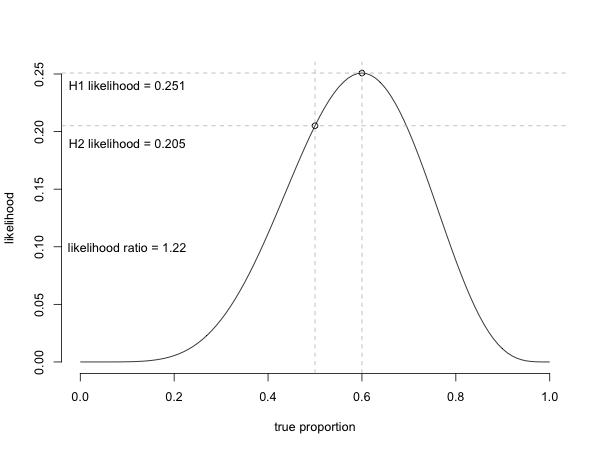
\includegraphics[width=.9\linewidth]{figures/coinFlip.png}
% Emacs 25.1.1 (Org mode 8.2.10)
\end{document}